\null
\vfill

\section{Introducci\'{o}n}
	El Spectrasoft es un software de c\'{o}digo abierto para el manejo del MiniScan XE Plus, el cual es usado en el diagn\'{o}stico de patolog\'{i}as dermatol\'{o}gicas en pacientes. Este software ofrece funciones de gesti\'{o}n de mediciones, historias m\'{e}dicas de pacientes y muestras. La vista principal del Spectrasoft es la mostrada en la figura 1.

\begin{figure}[H]
  \centering
  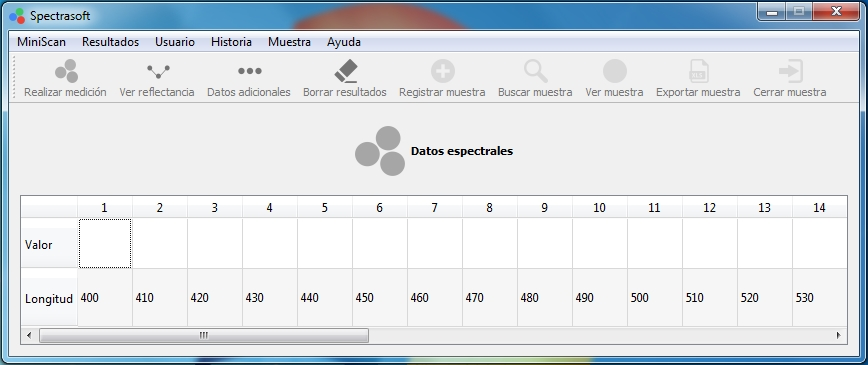
\includegraphics[width=1\linewidth]{./img/vista-principal.jpg}
\caption{Vista principal del Spectrasoft}
\end{figure}

\newpage

\section{Permisolog\'{i}a de los usuarios}

	Spectrasoft maneja tres roles de usuario: administradores, dermat\'{o}logos e investigadores. Si bien los tres roles comparten acciones comunes que pueden realizar, cada uno tiene permisos diferentes que lo distinguen de los dem\'{a}s. Estos permisos son descritos en la tabla 1.

\begin{table}[h]
		\small
		\caption[Permisolog\'{i}a de los usuarios]{Permisolog\'{i}a de los usuarios}
		\centering
		\setlength{\extrarowheight}{\altocelda}
		\begin{tabulary}{\anchotabla}{|c|J|}
			\hline
			\thead{\textbf{\small{Usuario}}} & \thead{\textbf{\small{Permisos}}}\\ \hline
			
			\textbf{Administrador} &
			
			Manejar el MiniScan XE Plus.
			
			Registrar, buscar, modificar y eliminar usuarios.
			
			Buscar y ver historias m\'{e}dicas de pacientes.
			
			Buscar y ver muestras de pacientes.\\ \hline
			
			\textbf{Dermat\'{o}logo} &
			
			Manejar el MiniScan XE Plus.
			
			Registrar, buscar, ver, modificar y eliminar historias m\'{e}dicas de pacientes.
			
			Registrar, buscar, ver, modificar y eliminar muestras de pacientes.\\ \hline
			
			\textbf{Investigador} &
			
			Manejar el MiniScan XE Plus.
			
			Buscar y ver historias m\'{e}dicas de pacientes.
			
			Buscar y ver muestras de pacientes.\\ \hline
		\end{tabulary}
	\end{table}

	Es importante destacar que todas las operaciones de registro, modificaci\'{o}n y eliminaci\'{o}n requieren de la contrase\~{n}a del usuario responsable de dicha operaci\'{o}n.
	
\newpage

\section{Manejo del MiniScan XE Plus}

	\subsection{Conectar y desconectar}
		Para conectar o desconectar el MiniScan XE Plus, entre al men\'{u} del MiniScan. Estas opciones son las ilustradas en la figura 2.

\begin{figure}[H]
\centering
\begin{subfigure}{.5\textwidth}
  \centering
  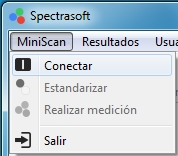
\includegraphics[width=.6\linewidth]{./img/conectar.jpg}
\end{subfigure}%
\begin{subfigure}{.5\textwidth}
  \centering
  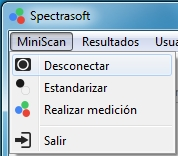
\includegraphics[width=.6\linewidth]{./img/desconectar.jpg}
\end{subfigure}
\caption{Conectar y desconectar MiniScan XE Plus}
\end{figure}

	\subsection{Calibrar}
		Entre al men\'{u} del Miniscan y seleccione la opci\'{o}n estandarizar. Prepare la trampa negra del Miniscan para su medici\'{o}n y seleccione listo, por \'{u}ltimo prepare la cer\'{a}mica blanca para su medici\'{o}n y seleccione listo. Todo esto se ilustra en la figura 3.
	
\begin{figure}[H]
\centering
\begin{subfigure}{.33\textwidth}
  \centering
  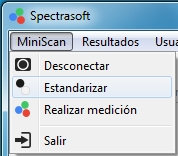
\includegraphics[width=.9\linewidth]{./img/estandarizar.jpg}
\end{subfigure}%
\centering
\begin{subfigure}{.33\textwidth}
  \centering
  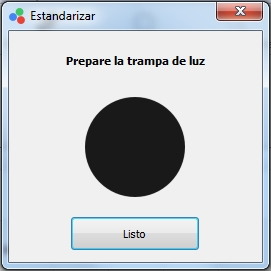
\includegraphics[width=.9\linewidth]{./img/estandarizar-negro.jpg}
\end{subfigure}%
\begin{subfigure}{.33\textwidth}
  \centering
  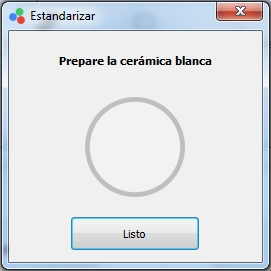
\includegraphics[width=.9\linewidth]{./img/estandarizar-blanco.jpg}
\end{subfigure}
\caption{Calibrar el MiniScan XE Plus}
\end{figure}

\section{Gesti\'{o}n de mediciones}
	
	\subsection{Realizar una medici\'{o}n}
	
	Entre al men\'{u} del MiniScan, o bien seleccione la opci\'{o}n directamente de la barra de herramientras. Estas opciones son las ilustradas en la figura 4.
	
\begin{figure}[H]
\centering
\begin{subfigure}{.5\textwidth}
  \centering
  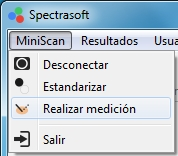
\includegraphics[width=.6\linewidth]{./img/medir-menu.jpg}
\end{subfigure}%
\begin{subfigure}{.5\textwidth}
  \centering
  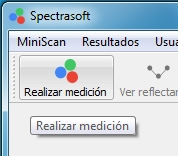
\includegraphics[width=.6\linewidth]{./img/medir-barra.jpg}
\end{subfigure}
\caption{Realizar medici\'{o}n}
\end{figure}

	\subsection{Consultar y borrar resultados de una medici\'{o}n}
	
	Los datos espectrales de una medici\'{o}n y los resultados relacionados con la misma aparecen se muestran en las figuras 5 y 6.
	
\begin{figure}[H]
  \centering
  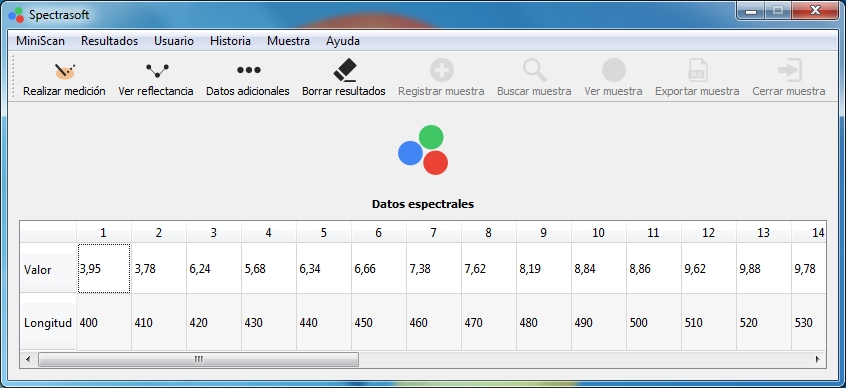
\includegraphics[width=1\linewidth]{./img/resultados.jpg}
\caption{Datos de una medici\'{o}n}
\end{figure}

\begin{figure}[H]
  \centering
  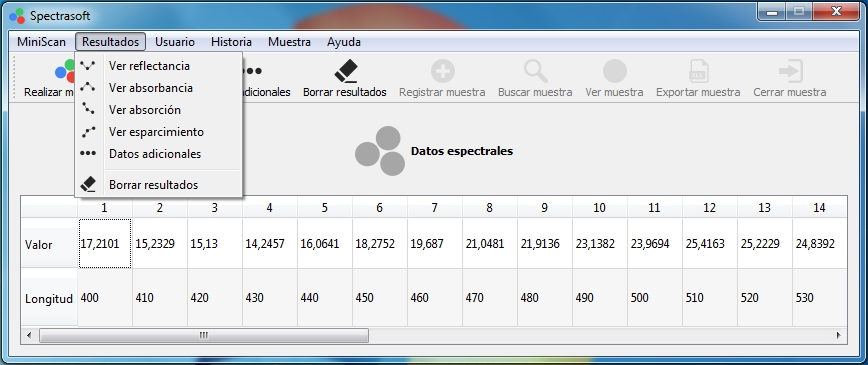
\includegraphics[width=1\linewidth]{./img/resultados-menu.jpg}
\caption{Men\'{u} de resultados de una medici\'{o}n}
\end{figure}

\section{Gesti\'{o}n de sesiones}

	\subsection{Iniciar sesi\'{o}n}
	
	Para iniciar sesi\'{o}n entre al men\'{u} de usuario y seleccione la opci\'{o}n iniciar sesi\'{o}n. Debe ingresar su c\'{e}dula de identidad y su contrase\~{n}a. Esto es ilustrado en la figura 7.
	
\begin{figure}[H]
  \centering
  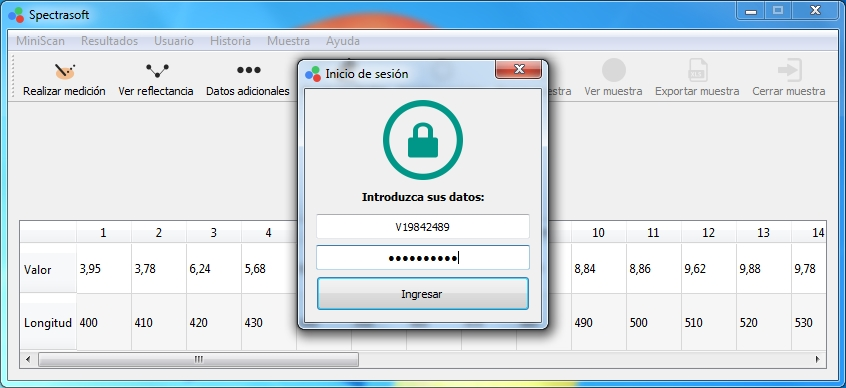
\includegraphics[width=1\linewidth]{./img/inicio-sesion.jpg}
\caption{Iniciar sesi\'{o}n}
\end{figure}
	
	\subsection{Ver informaci\'{o}n del usuario}
	
	Seleccione la opci\'{o}n ver usuario, ubicada en el men\'{u} de usuario. El men\'{u} de usuario y la ventana de informaci\'{o}n son ilustrados en las figuras 8 y 9.

\begin{figure}[H]
  \centering
  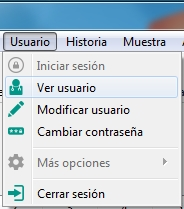
\includegraphics[width=.3\linewidth]{./img/menu-usuario.jpg}
\caption{Men\'{u} de usuario}
\end{figure}

\begin{figure}[H]
  \centering
  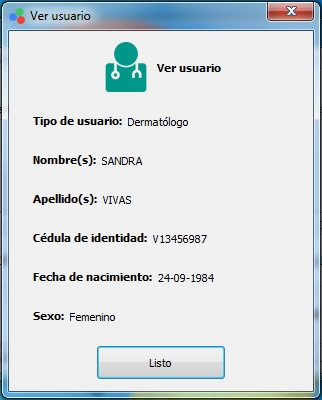
\includegraphics[width=.5\linewidth]{./img/ver-usuario.jpg}
\caption{Ver usuario}
\end{figure}

\newpage

	\subsection{Modificar informaci\'{o}n del usuario}
	
	Seleccione la opci\'{o}n modificar usuario, ubicada en el men\'{u} de usuario. La ventana para modificar el usuario es ilustrada en la figura 10.

	\subsection{Cambiar contrase\~{n}a del usuario}
	
	Seleccione la opci\'{o}n cambiar contrase\~{n}a, ubicada en el men\'{u} de usuario. Debe ingresar la contrase\~{n}a actual del usuario y la nueva contrase\~{n}a (dos veces) para poder realizar el cambio. La ventana para realizar esta operaci\'{o}n se ilustra en la figura 11.

\begin{figure}[H]
\centering
\begin{minipage}{.5\textwidth}
  \centering
  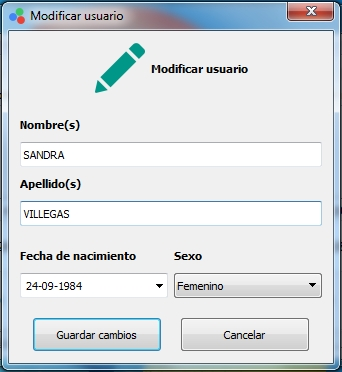
\includegraphics[width=.9\linewidth]{./img/modificar-usuario.jpg}
  \captionof{figure}{Modificar usuario}
  \label{fig:test1}
\end{minipage}%
\begin{minipage}{.5\textwidth}
  \centering
  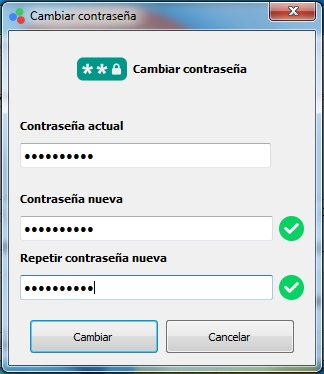
\includegraphics[width=.9\linewidth]{./img/cambiar-clave.jpg}
  \captionof{figure}{Cambiar contrase\~{n}a}
  \label{fig:test2}
\end{minipage}
\end{figure}

	\subsection{Cerrar sesi\'{o}n}
	
	Seleccione la opci\'{o}n cerrar sesi\'{o}n, ubicada en el men\'{u} usuario.

\newpage

\section{Gesti\'{o}n de historias}

	\subsection{Registrar historia}
	
	Seleccione la opci\'{o}n registrar historia, ubicada en el men\'{u} historia. Solo los usuarios dermat\'{o}logos pueden registrar una historia m\'{e}dica. El men\'{u} de historia y la ventana de registro se ilustran en las figuras 12 y 13.

\begin{figure}[H]
  \centering
  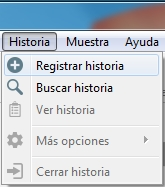
\includegraphics[width=.3\linewidth]{./img/menu-historia.jpg}
\caption{Men\'{u} historia}
\end{figure}

\begin{figure}[H]
  \centering
  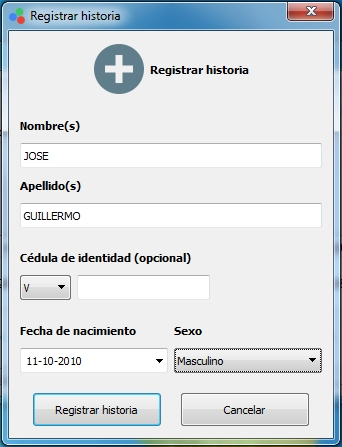
\includegraphics[width=.4\linewidth]{./img/registrar-historia.jpg}
\caption{Resgistrar historia}
\end{figure}

	\subsection{Buscar historia}
	
	En el men\'{u} de historia, seleccione la opci\'{o}n buscar historia. Esta ventana permite filtrar la b\'{u}squeda de historias empleando ciertos criterios. Para abrir la historia, seleccionela en la lista de historias y por \'{u}ltimo seleccione la opci\'{o}n abrir historia. Esta ventana se ilustra en la figura 14.
	
\begin{figure}[H]
  \centering
  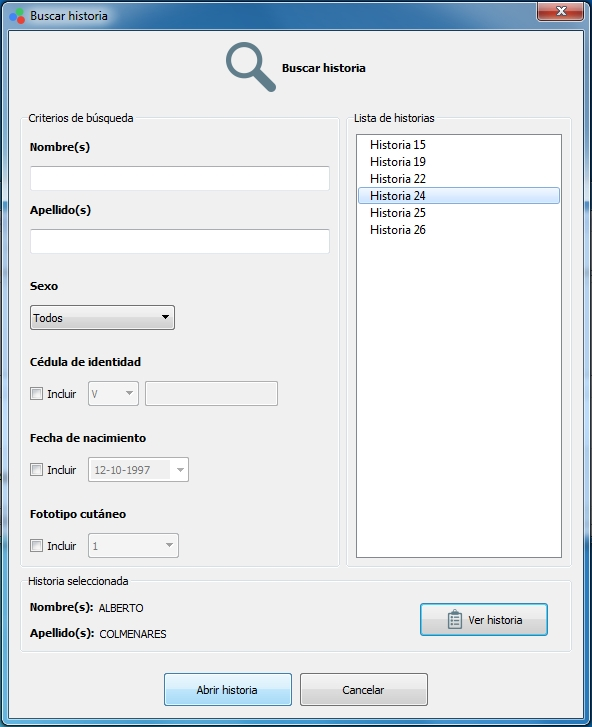
\includegraphics[width=.9\linewidth]{./img/buscar-historia.jpg}
\caption{Buscar historia}
\end{figure}
	
	\subsection{Ver historia}
	
	Seleccione la opci\'{o}n ver historia, ubicada en el men\'{u} historia. Esta ventana es ilustrada en la figura 15.
	
\begin{figure}[H]
  \centering
  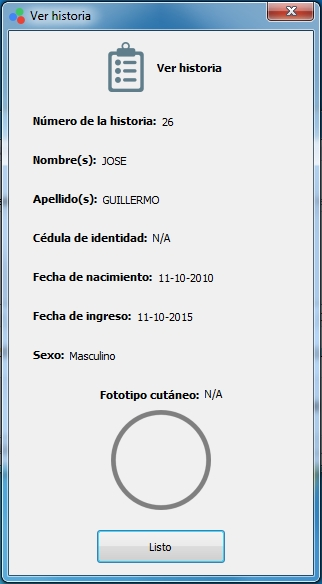
\includegraphics[width=.6\linewidth]{./img/ver-historia1.jpg}
\caption{Ver historia}
\end{figure}
		
	\subsection{Modificar historia}
	
	Seleccione la opci\'{o}n modificar historia, ubicada en el submen\'{u} m\'{a}s opciones, dentro del men\'{u} historia. Esta ventana se ilustra en la figura 16.
	
	\subsection{Eliminar historia}
	
	Seleccione la opci\'{o}n eliminar historia, ubicada en el submen\'{u} m\'{a}s opciones, dentro del men\'{u} historia. Esta ventana se ilustra en la figura 17.
	
\begin{figure}[H]
\centering
\begin{minipage}{.5\textwidth}
  \centering
  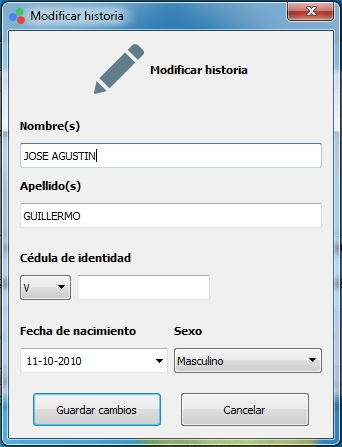
\includegraphics[width=.9\linewidth]{./img/modificar-historia.jpg}
  \captionof{figure}{Modificar historia}
  \label{fig:test1}
\end{minipage}%
\begin{minipage}{.5\textwidth}
  \centering
  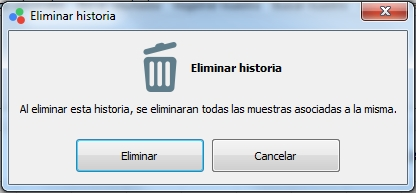
\includegraphics[width=1\linewidth]{./img/eliminar-historia.jpg}
  \captionof{figure}{Eliminar historia}
  \label{fig:test2}
\end{minipage}
\end{figure}

	\subsection{Cerrar historia}
	
	Seleccione la opci\'{o}n cerrar historia, ubicada en el men\'{u} historia.

\newpage

\section{Gesti\'{o}n de muestras}

	\subsection{Registrar muestra}
	
	Seleccione la opci\'{o}n registrar muestra, ubicada en el men\'{u} de muestra (tambi\'{e}n disponible en la barra de herramientas). En la ventana de registro aparecer\'{a}n dos tipos de muestra que se pueden registrar, fototipo y lesi\'{o}n. Solo se puede registrar una muestra si el usuario es dermat\'{o}logo, si hay una historia m\'{e}dica cargada y si se realiz\'{o} una medici\'{o}n nueva. El men\'{u} muestra y la ventana de tipos de muestra se ilustran en las figuras 18 y 19.
	
\begin{figure}[H]
  \centering
  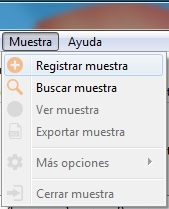
\includegraphics[width=.3\linewidth]{./img/menu-muestra.jpg}
\caption{Men\'{u} muestra}
\end{figure}

\begin{figure}[H]
  \centering
  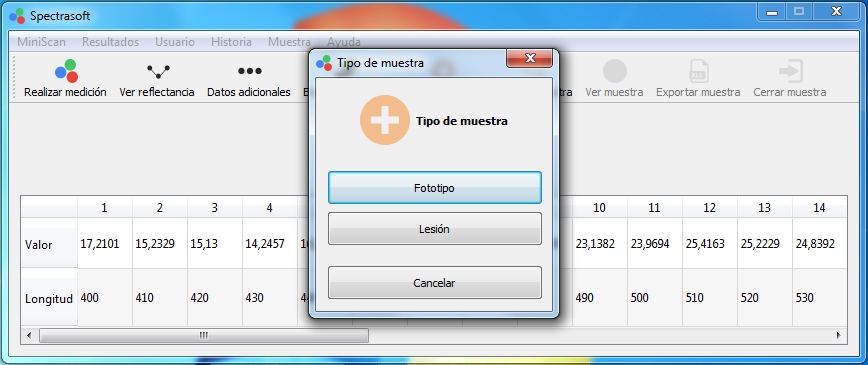
\includegraphics[width=.9\linewidth]{./img/tipo-muestra.jpg}
\caption{Tipos de muestra}
\end{figure}
	
		\subsubsection{Registrar fototipo}
		
		En la ventana para registrar un fototipo, debe especificar el \'{a}rea en donde se le est\'{a} tomando la muestra al paciente, y se debe seleccionar el fototipo, en la opci\'{o}n clasificar fototipo. Esta ventana se puede apreciar en la figura 20.
		
\begin{figure}[H]
  \centering
  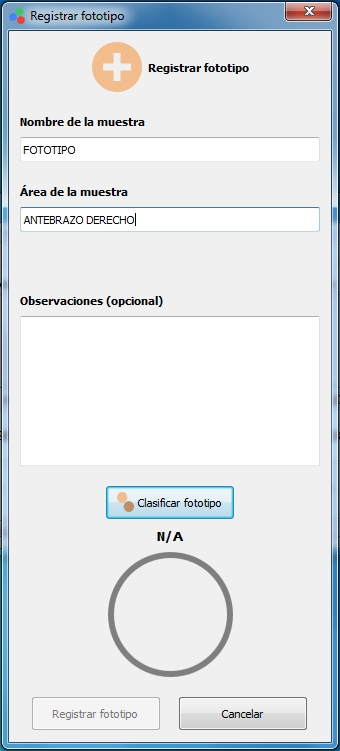
\includegraphics[width=.5\linewidth]{./img/registrar-fototipo1.jpg}
\caption{Registrar fototipo}
\end{figure}

		En la ventana de clasificaci\'{o}n del fototipo aparecer\'{a} el fototipo recomendado para la muestra dada, y ser\'{a} necesario elegir el fototipo que se desea registrar. Esto es ilustrado en la figura 21.
		
		
\begin{figure}[H]
  \centering
  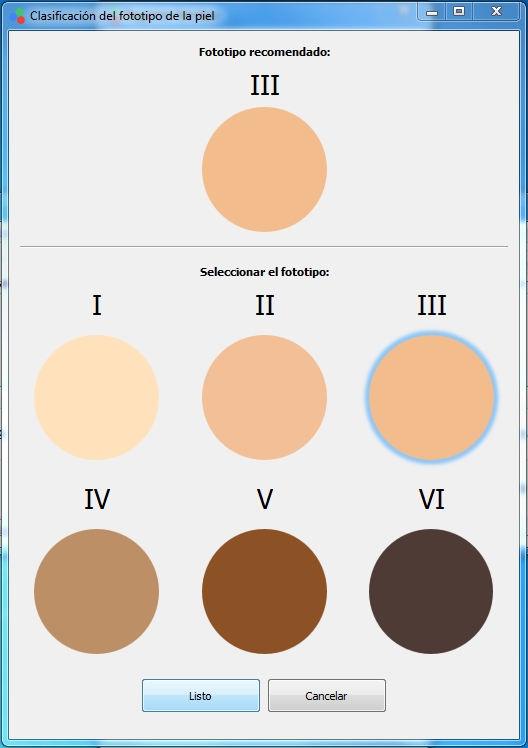
\includegraphics[width=.8\linewidth]{./img/fototipo.jpg}
\caption{Clasificar fototipo}
\end{figure}
\newpage
	Luego de haber elegido el fototipo, aparecer\'{a} la ventana de registro nuevamente, con el fototipo elegido actualizado; por \'{u}ltimo, seleccione registrar fototipo. Esto es ilustrado en la figura 22.

\begin{figure}[H]
  \centering
  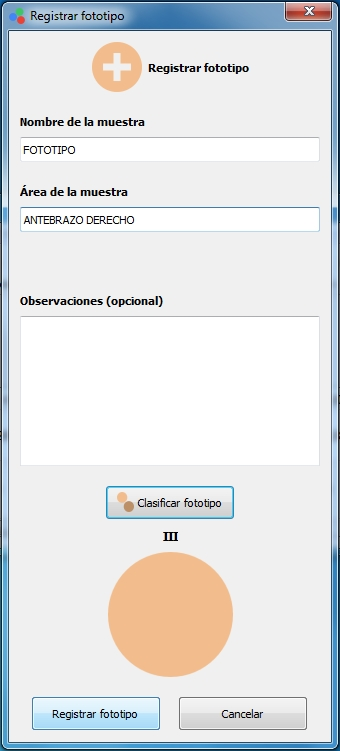
\includegraphics[width=.5\linewidth]{./img/registrar-fototipo2.jpg}
\caption{Registrar fototipo}
\end{figure}
\newpage		
		\subsubsection{Registrar lesi\'{o}n}
			En la ventana de registrar lesi\'{o}n, debe especificar el nombre de la lesi\'{o}n y el \'{a}rea en donde se est\'{a} tomando la muestra de la misma. Esta ventana se puede apreciar en la figura 23.		
		
		
\begin{figure}[H]
  \centering
  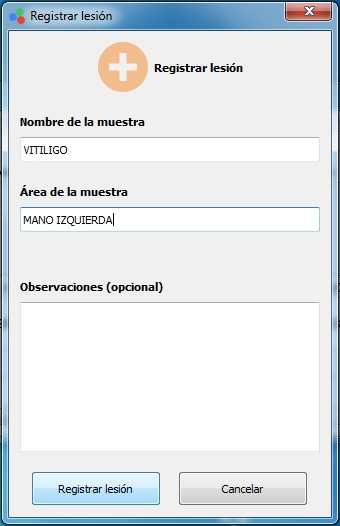
\includegraphics[width=.6\linewidth]{./img/registrar-lesion.jpg}
\caption{Registrar lesi\'{o}n}
\end{figure}
	
	\subsection{Buscar muestra}
	
		Seleccione la opci\'{o}n buscar muestra, ubicada en el men\'{u} de muestra (tambi\'{e}n disponible en la barra de herramientas). Esta ventana permite filtrar la b\'{u}squeda de las muestras pertenecientes a la historia que est\'{e} cargada en ese momento, empleando ciertos criterios. Para abrir la muestra, seleccionela en la lista de muestras y por \'{u}ltimo seleccione la opci\'{o}n abrir muestra. Esta ventana se ilustra en la figura 24.
		
\begin{figure}[H]
  \centering
  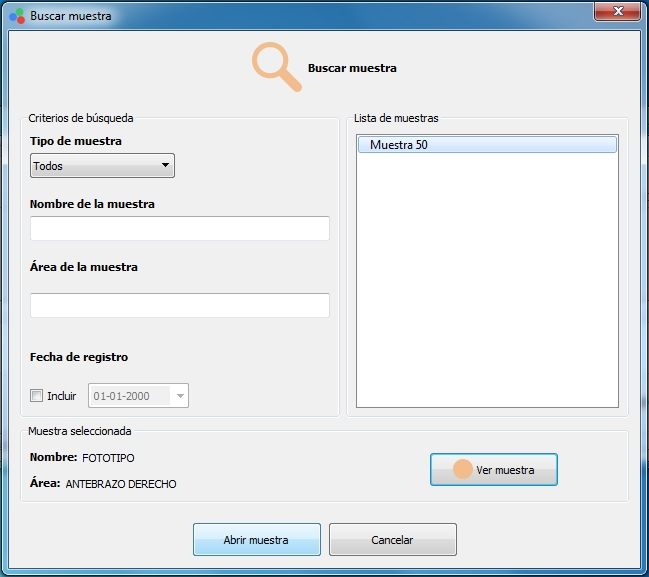
\includegraphics[width=.9\linewidth]{./img/buscar-muestra.jpg}
\caption{Buscar muestra}
\end{figure}
	
	\subsection{Ver muestra}
	
	Seleccione la opci\'{o}n ver muestra, ubicada en el men\'{u} de muestra (tambi\'{e}n disponible en la barra de herramientas). Esta ventana se ilustra en la figura 25.
	
\begin{figure}[H]
  \centering
  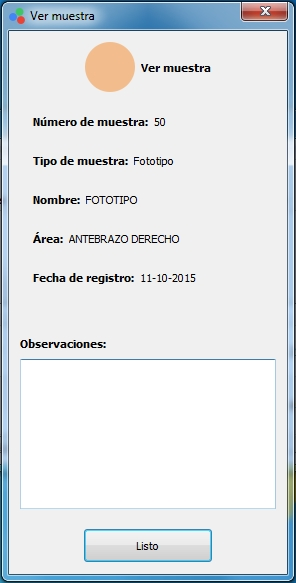
\includegraphics[width=.5\linewidth]{./img/ver-muestra.jpg}
\caption{Ver muestra}
\end{figure}

	\subsection{Exportar muestra}
	
	Seleccione la opci\'{o}n exportar muestra, ubicada en el men\'{u} de muestra (tambi\'{e}n disponible en la barra de herramientas). Estas opciones se ilustran en la figura 26.
	
\begin{figure}[H]
\centering
\begin{subfigure}{.5\textwidth}
  \centering
  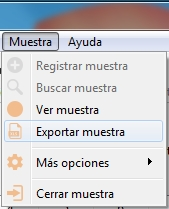
\includegraphics[width=.6\linewidth]{./img/exportar-menu.jpg}
\end{subfigure}%
\begin{subfigure}{.5\textwidth}
  \centering
  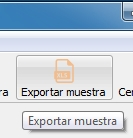
\includegraphics[width=.45\linewidth]{./img/exportar-barra.jpg}
\end{subfigure}
\caption{Exportar muestra}
\end{figure}

	La muestra se exporta en el escritorio a un archivo .xlsx, que puede abrirse y modificarse con cualquier programa que maneje hojas de c\'{a}lculo.

	\subsection{Modificar muestra}
	
	Seleccione la opci\'{o}n modificar muestra, ubicada en el submen\'{u} m\'{a}s opciones, dentro del men\'{u} muestra. Esta ventana se ilustra en la figura 27.
	
	\subsection{Eliminar muestra}
	
	Seleccione la opci\'{o}n eliminar muestra, ubicada en el submen\'{u} m\'{a}s opciones, dentro del men\'{u} muestra. Esta ventana se ilustra en la figura 28.
	
\begin{figure}[H]
\centering
\begin{minipage}{.5\textwidth}
  \centering
  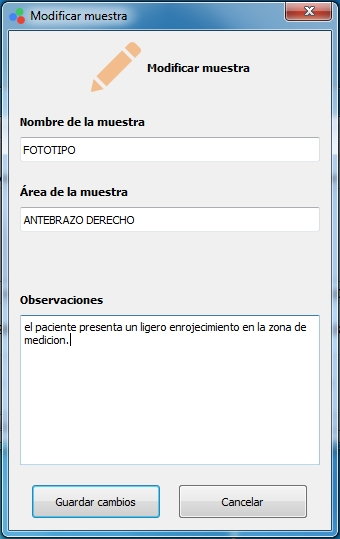
\includegraphics[width=.9\linewidth]{./img/modificar-muestra.jpg}
  \captionof{figure}{Modificar muestra}
  \label{fig:test1}
\end{minipage}%
\begin{minipage}{.5\textwidth}
  \centering
  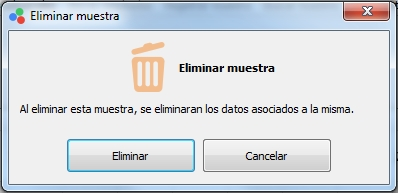
\includegraphics[width=1\linewidth]{./img/eliminar-muestra.jpg}
  \captionof{figure}{Eliminar muestra}
  \label{fig:test2}
\end{minipage}
\end{figure}

	\subsection{Cerrar muestra}
	
	Seleccione la opci\'{o}n cerrar muestra, ubicada en el men\'{u} muestra.

\newpage

\section{Gesti\'{o}n de usuarios}

	\subsection{Registrar usuario}
	
	Seleccione la opci\'{o}n registrar usuario, ubicada en el submen\'{u} m\'{a}s opciones, dentro del men\'{u} usuario. Esta ventana es ilustrada en la figura 29.
	
\begin{figure}[H]
  \centering
  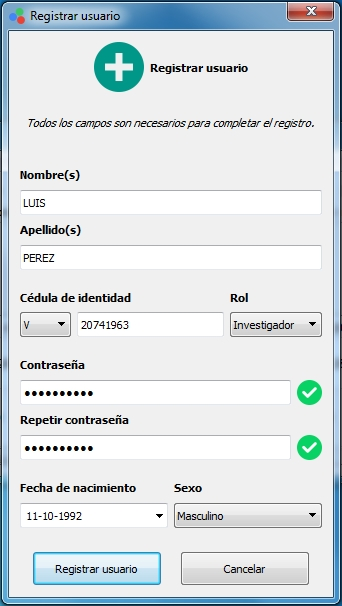
\includegraphics[width=.6\linewidth]{./img/registrar-usuario.jpg}
\caption{Registrar usuario}
\end{figure}
	
	\subsection{Administrar usuarios}
	
	Seleccione la opci\'{o}n administrar usuarios, ubicada en el submen\'{u} m\'{a}s opciones, dentro del men\'{u} usuario. Administrar usuarios permite cambiar sus roles, cambiar sus contrase\~{n}as y eliminarlos. Esta ventana es ilustrada en la figura 30.
	
\begin{figure}[H]
  \centering
  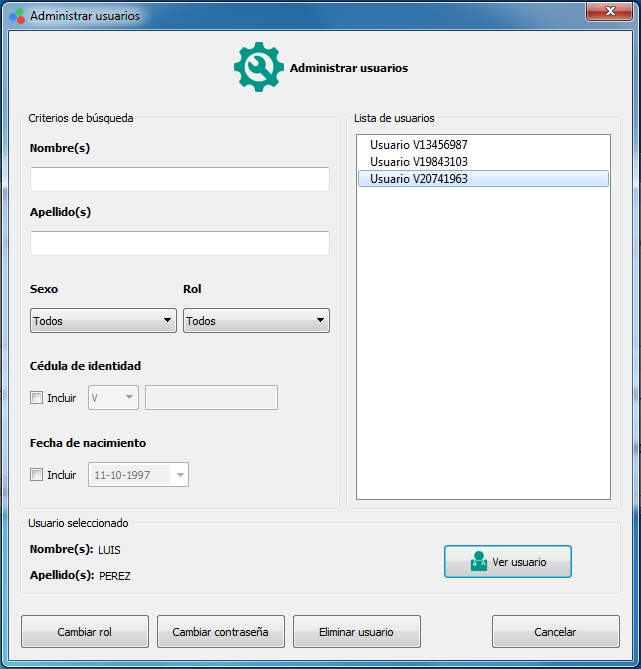
\includegraphics[width=1\linewidth]{./img/administrar-usuarios.jpg}
\caption{Administrar usuarios}
\end{figure}
	
		\subsubsection{Cambiar rol}
		
		Una vez haya seleccionado un usuario de la lista de usuarios, seleccione la opci\'{o}n cambiar rol. Esta ventana es ilustrada en la figura 31.
		
\begin{figure}[H]
  \centering
  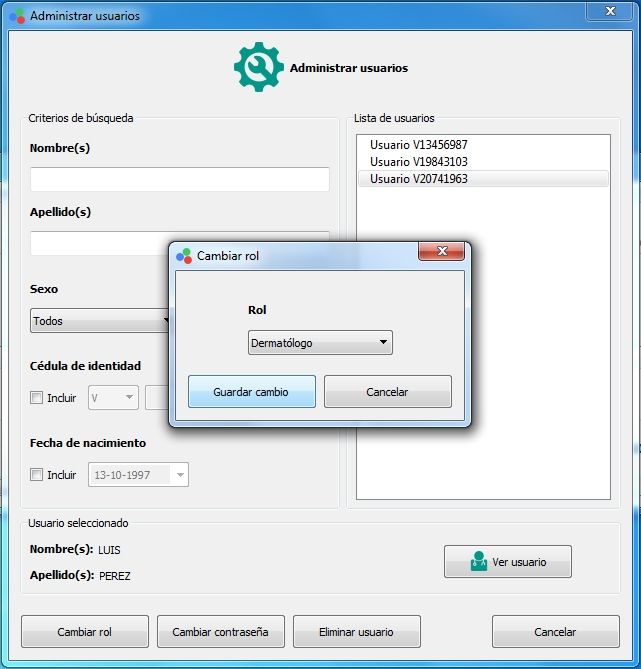
\includegraphics[width=1\linewidth]{./img/administrar-rol.jpg}
\caption{Cambiar rol}
\end{figure}
		
		\subsubsection{Cambiar contrase\~{n}a}
		
		Una vez haya seleccionado un usuario de la lista de usuarios, seleccione la opci\'{o}n cambiar contrase\~{n}a. Esta opci\'{o}n requiere de la contrase\~{n}a del administrador que este realizando la operaci\'{o}n, y de la nueva contrase\~{n}a para el usuario. Esto es ilustrado en la figura 32.
		
\begin{figure}[H]
  \centering
  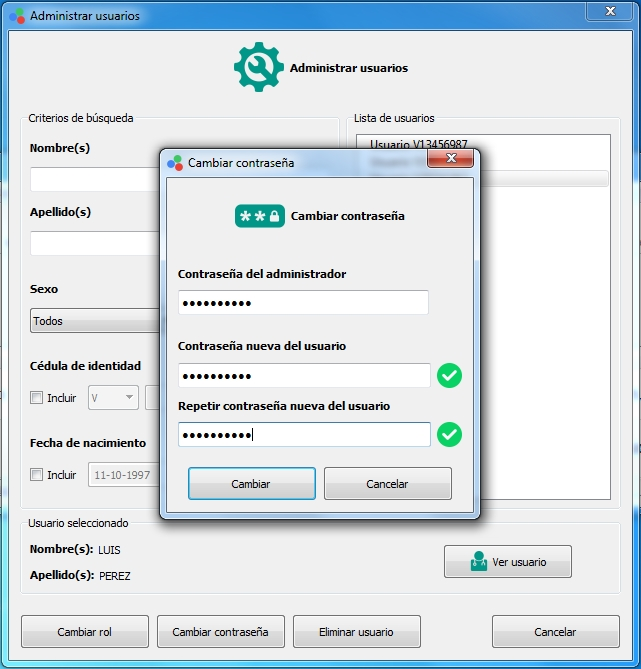
\includegraphics[width=1\linewidth]{./img/administrar-clave.jpg}
\caption{Cambiar contrase\~{n}a}
\end{figure}
		
		\subsubsection{Eliminar usuario}
		
		Una vez haya seleccionado un usuario de la lista de usuarios, seleccione la opci\'{o}n eliminar usuario. Esta opci\'{o}n solo se puede realizar con usuarios que no sean administradores. Esta opci\'{o}n es ilustrada en la figura 33.
		
\begin{figure}[H]
  \centering
  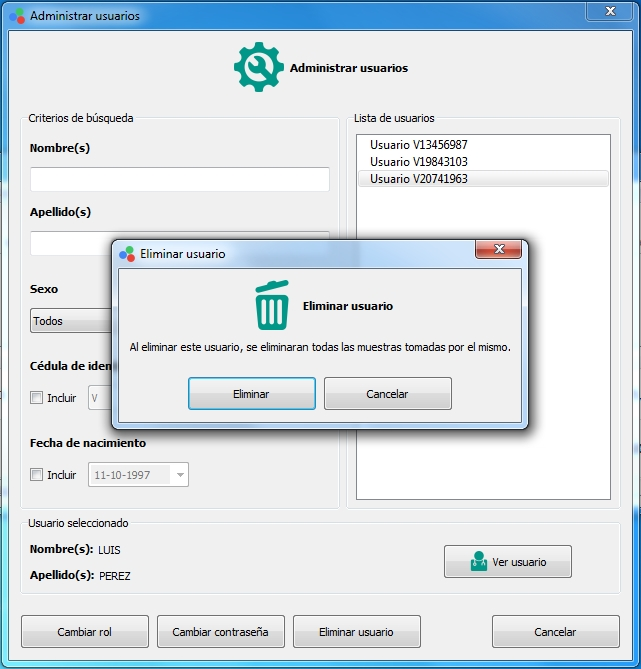
\includegraphics[width=1\linewidth]{./img/administrar-eliminar.jpg}
\caption{Eliminar usuario}
\end{figure}